\section{Versuchsdurchführung}

 \subsection{Durchlassfilter als Frequenzfilter}
Zur Überprüfung der Funktionsweise eines Frequenzfilters wurde zunächst die Schaltung aus
Abb. xyz wie in Abb. abc realisiert. Nach anfänglichen Problemen mit der richtigen Dimensionierung 
der verwendeten Spule haben wir schließlich eine Spule "Leybold 56214" mit 500 Windungen und einer 
Induktivität von 9 mH verwendet, wobei hier das Augenmerk auf einer möglichst geringen Windungszahl 
liegt, um den in anderen Bauteilen angesiedelten Widerstand möglichst gering zu halten. Dieser liegt 
für die Spule bei angegebenen $ 2,5  \Omega $, was durch Messung bestätigt wurde. Auf der anderen Seite 
musste auch eine hinreichend große Induktivität garantiert werden, damit die Resonanzfrequenz, in deren 
Umgebungen die Messungen stattfanden, in einem gut erfassbaren Bereich lagen. Weiter wurde ein 
Plastikfolienkondensator der Firma "WIMA" der Kapazität 0,22 mF sowie in einem zweiten Teilversuch
ein Kondensator gleicher Bauart, allerdings mit 4,7 mF Kapazität verwendet. Ebenfalls als variabel
wurde der Widerstand gewählt, wobei hier ein Widerstandskasten, mit dem Widerstände im Bereich von $ 
1  \Omega $ bis mehrere $ M \Omega $ zugeschaltet werden können, verwendet wurde. \\
Zur Erzeugung der Eingangsspannung wurde zunächst ein Frequenzgenerator der Marke Hameg (Programmable 
15 MHz Function Generator, HM8131/2) verwendet, zur Vereinfachung und Automatisierung der Messung wurde 
dieser allerdings durch das Power-Cassy ersetzt.
Die Messung der über dem Widerstand abfallenden Ausgangsspannung wurde bei einem ersten Aufbau mit 
einem Oszilloskop (Tektronix TDS 2024 100mHz, PPL28/2/001) durchgeführt. Hierbei stellte sich allerdings 
heraus, dass die Messungen etwas an Genauigkeit zu wünschen übrig ließen. Bei der tatschlichen 
Durchführung des Experiments haben wir stattdessen das Sensor-Cassy zugeschalten; Vorteil hierbei ist 
klar die direkte Übertragung der Daten in die Cassy-Software.\\
\\
\subsection{Sperrfilter als Frequenzfilter}
Für die Abwandlung des Durchlassfilters zu einem Frequenzfilter müssen lediglich Kapazität und
Induktivität parallel anstatt in Reihe geschaltet werden. Für diesen Versuch wurden mit Ausnahme des
Widerstandes die selben Bauteile erhalten. Um für dieses Experiment den teilweise recht schwach 
ausgebildeten Peak deutlicher sichtbar zu machen, also eine geringere Breite zu erreichen, wurde 
allerdings die Widerstandsbox durch einen einfachen Steckwiderstand, wie etwa in Abb. xyz ersetzt. 
Grund dafür ist, dass die Widerstandsbox insbesondere bei den kleinsten Widerständen einen zu großen 
Widerstand liefert.


\begin{figure}
\centering
    \subcaptionbox{Durchlassfilter\label{img:durchlass}}[.4\linewidth]
            {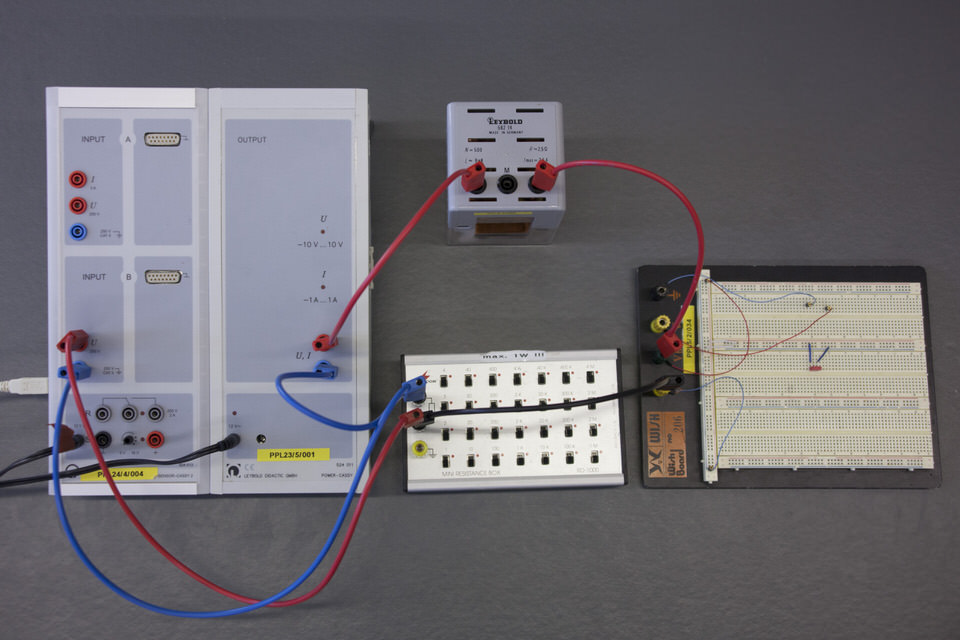
\includegraphics[width=.4\textwidth]{images/durchlassfilter.jpg}}
    \subcaptionbox{Sperrfilter\label{img:sperr}}[.4\linewidth]
            {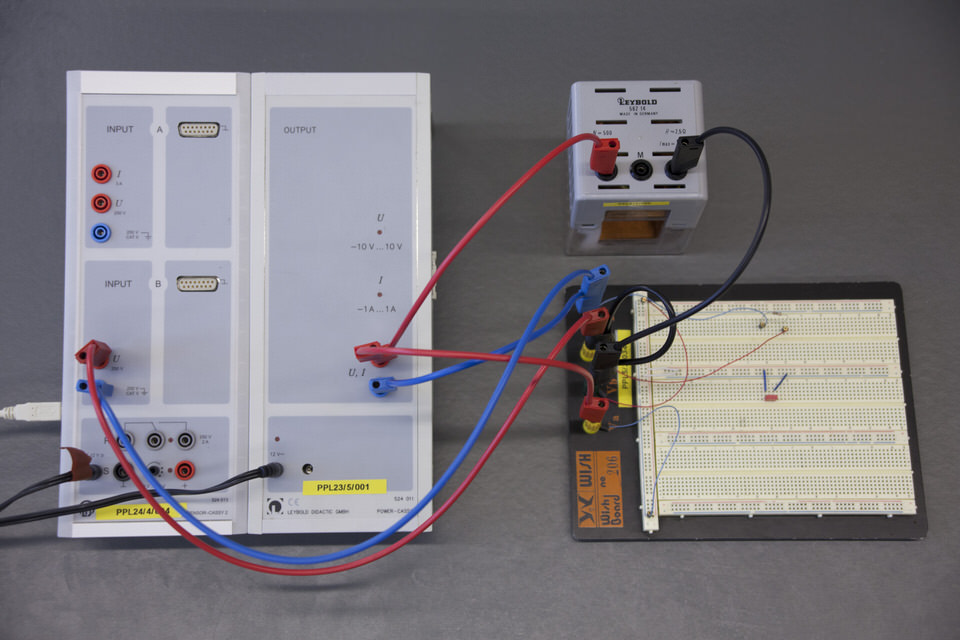
\includegraphics[width=.4\textwidth]{images/sperrfilter.jpg}}
\caption{Fotos der Versuchsaufbauten}
\end{figure}

